% Digital Logic Report Template
% Created: 2020-01-10, John Miller

%==========================================================
%=========== Document Setup  ==============================

% Formatting defined by class file
\documentclass[11pt]{article}

% ---- Document formatting ----
\usepackage[margin=1in]{geometry}	% Narrower margins
\usepackage{booktabs}				% Nice formatting of tables
\usepackage{graphicx}				% Ability to include graphics

%\setlength\parindent{0pt}	% Do not indent first line of paragraphs 
\usepackage[parfill]{parskip}		% Line space b/w paragraphs
%	parfill option prevents last line of pgrph from being fully justified

% Parskip package adds too much space around titles, fix with this
\RequirePackage{titlesec}
\titlespacing\section{0pt}{8pt plus 4pt minus 2pt}{3pt plus 2pt minus 2pt}
\titlespacing\subsection{0pt}{4pt plus 4pt minus 2pt}{-2pt plus 2pt minus 2pt}
\titlespacing\subsubsection{0pt}{2pt plus 4pt minus 2pt}{-6pt plus 2pt minus 2pt}

% ---- Hyperlinks ----
\usepackage[colorlinks=true,urlcolor=blue]{hyperref}	% For URL's. Automatically links internal references.

% ---- Code listings ----
\usepackage{listings} 					% Nice code layout and inclusion
\usepackage[usenames,dvipsnames]{xcolor}	% Colors (needs to be defined before using colors)

% Define custom colors for listings
\definecolor{listinggray}{gray}{0.98}		% Listings background color
\definecolor{rulegray}{gray}{0.7}			% Listings rule/frame color

% Style for Verilog
\lstdefinestyle{Verilog}{
	language=Verilog,					% Verilog
	backgroundcolor=\color{listinggray},	% light gray background
	rulecolor=\color{blue}, 			% blue frame lines
	frame=tb,							% lines above & below
	linewidth=\columnwidth, 			% set line width
	basicstyle=\small\ttfamily,	% basic font style that is used for the code	
	breaklines=true, 					% allow breaking across columns/pages
	tabsize=3,							% set tab size
	commentstyle=\color{gray},	% comments in italic 
	stringstyle=\upshape,				% strings are printed in normal font
	showspaces=false,					% don't underscore spaces
}

% How to use: \Verilog[listing_options]{file}
\newcommand{\Verilog}[2][]{%
	\lstinputlisting[style=Verilog,#1]{#2}
}




%======================================================
%=========== Body  ====================================
\begin{document}

\title{ELC 2137 Lab \09: ALU}
\author{Spencer Stinson}

\maketitle


\section*{Summary}
In this lab, we created an arithmetic logic unit capable of 4 operations, and with room to program more operations into the program. By using our program, we are able to save a value so that we can perform these operations with just a few pushes of a button. We were able to do this by use of sequential and combinational logic and by using new latches and flip flops that we have been taught. 

\section*{Results}

\begin{figure}[ht]\centering
	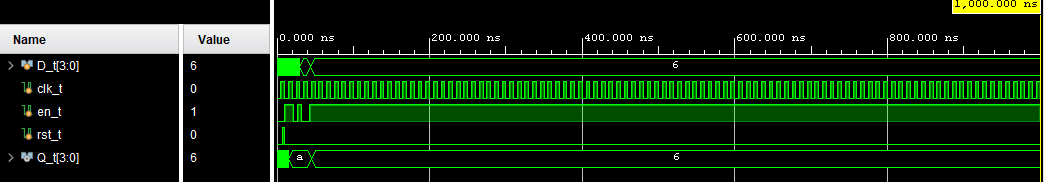
\includegraphics[width= \textwidth ]{regsw.png}
	\caption{register simulation waveform}
	\label{fig: regsw}
\end{figure}

\begin{figure}[ht]\centering
	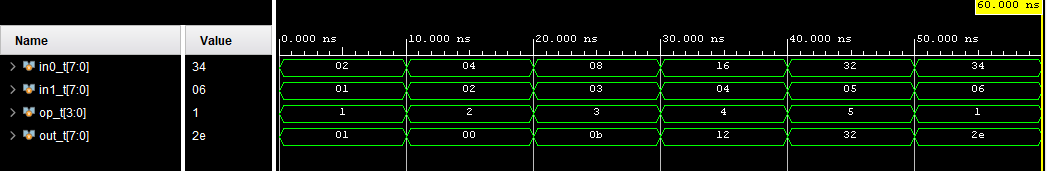
\includegraphics[width= \textwidth ]{alusw.png}
	\caption{alu simulation waveform}
	\label{fig: alusw}
\end{figure}

\begin{figure}[ht]\centering
	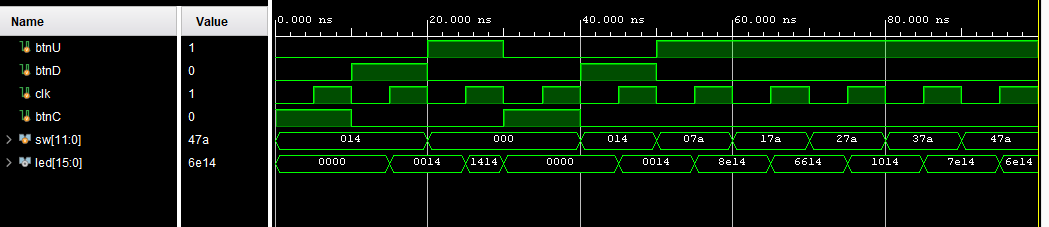
\includegraphics[width= \textwidth ]{swtls.png}
	\caption{top level simulation waveform}
	\label{fig: tlsw}
\end{figure}

\begin{figure}[ht]\centering
	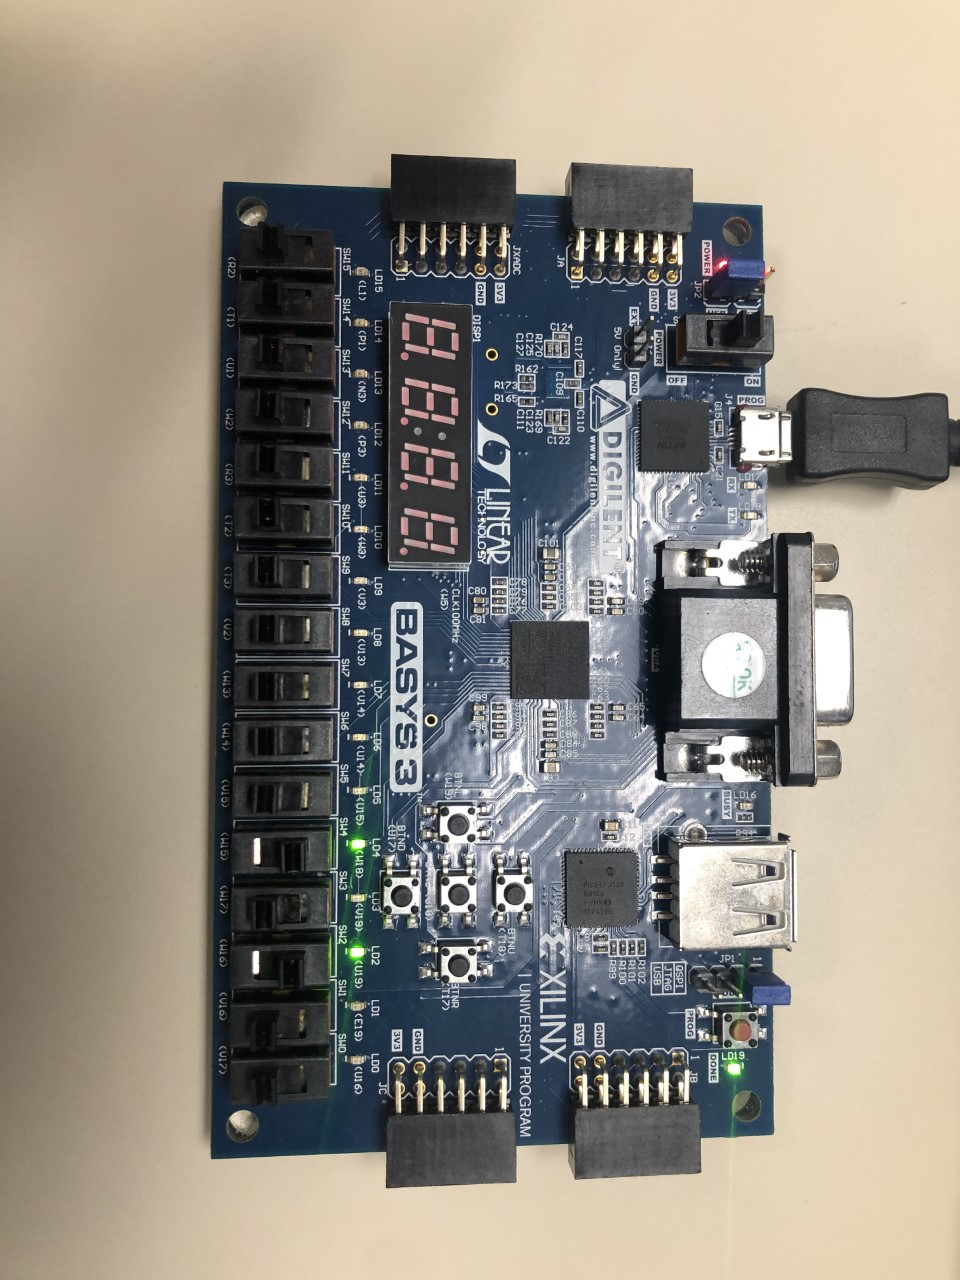
\includegraphics[width= \textwidth ]{bb1.png}
	\caption{14 displayed in hexidecimal}
	\label{fig: bb1}
\end{figure}

\begin{figure}[ht]\centering
	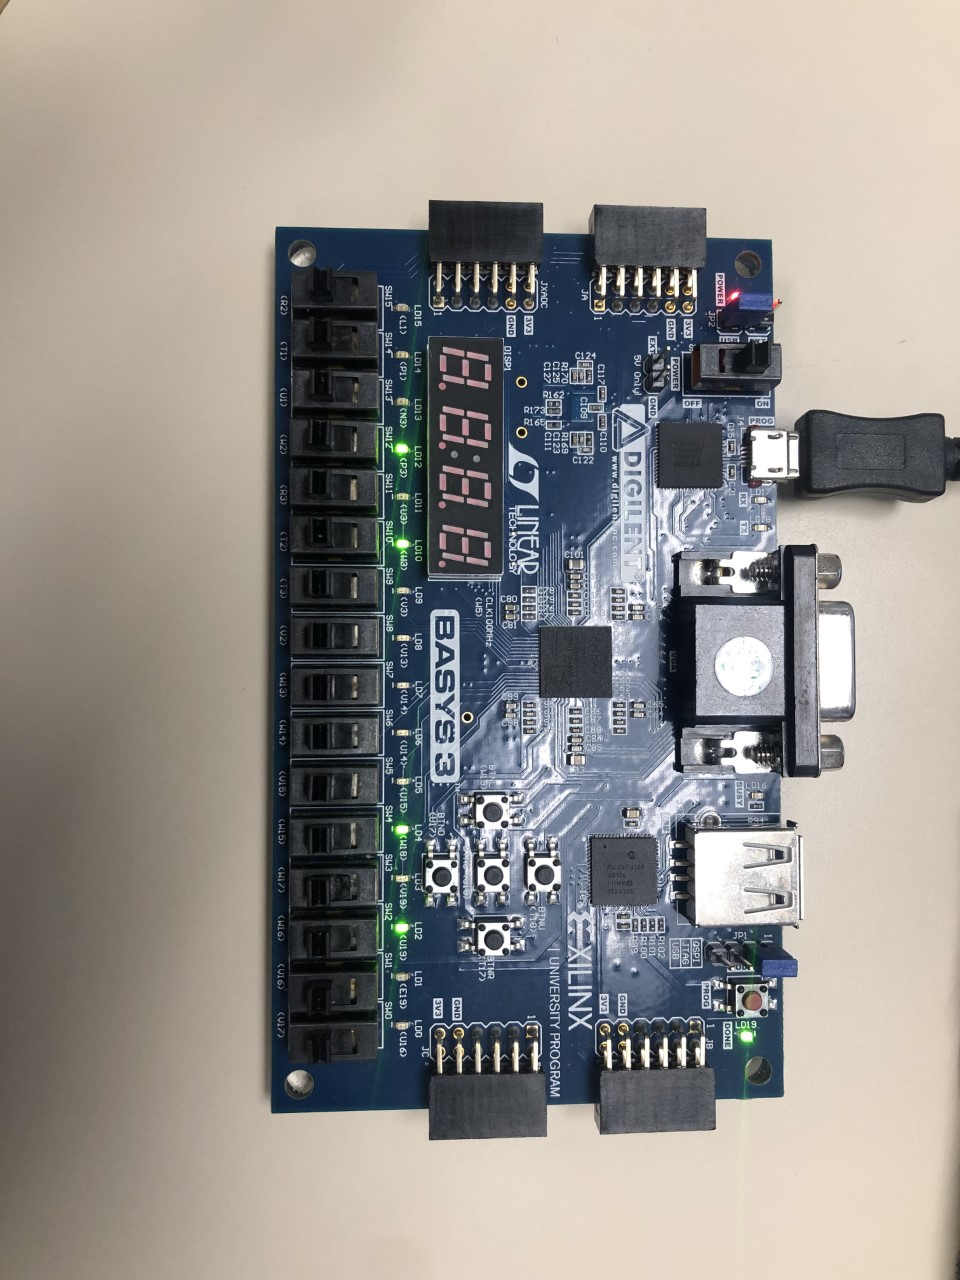
\includegraphics[width= \textwidth ]{bb2.png}
	\caption{1414 displayed in leds}
	\label{fig: bb2}
\end{figure}

\begin{figure}[ht]\centering
	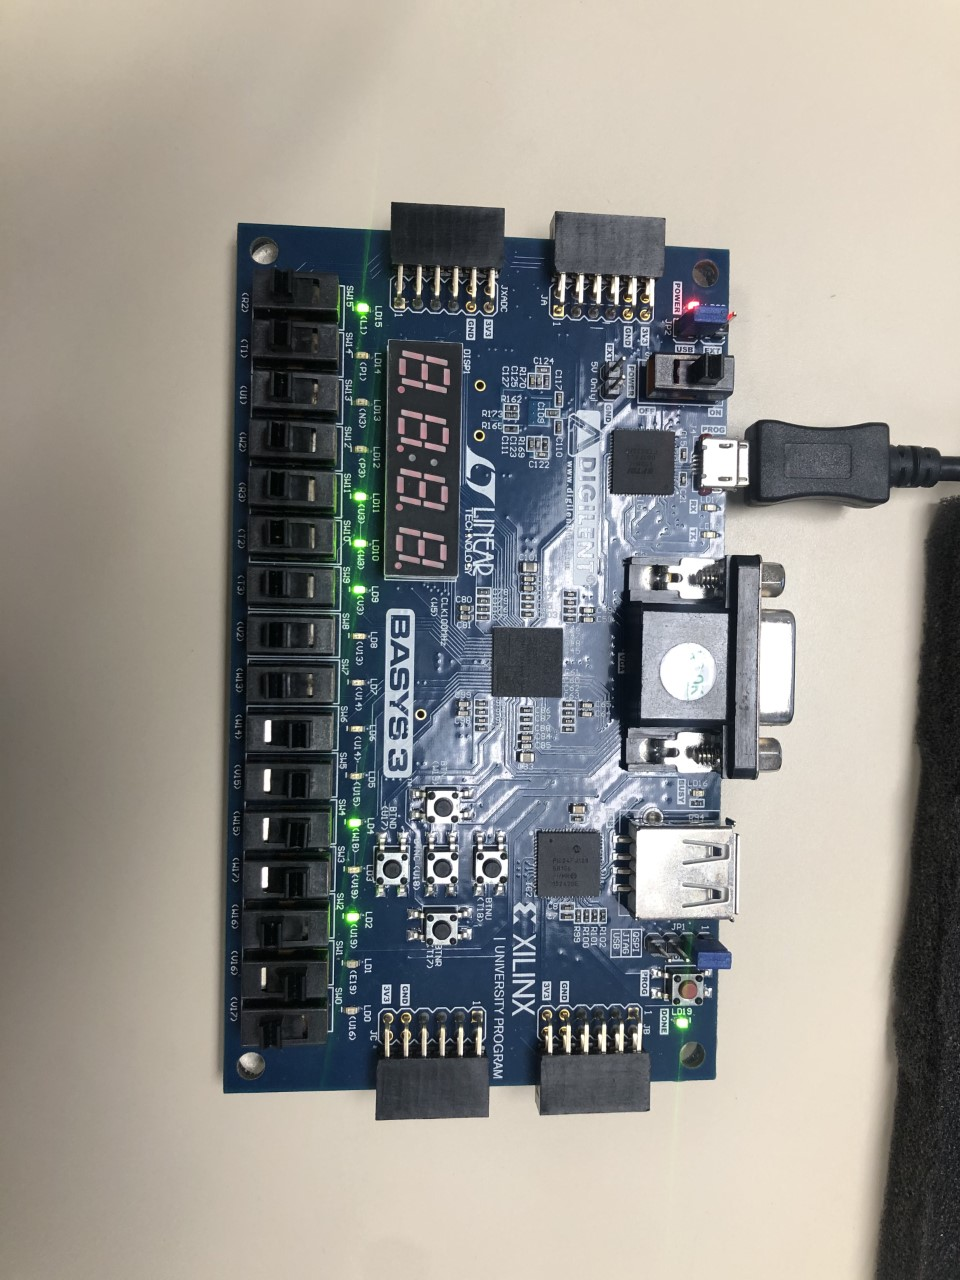
\includegraphics[width= \textwidth ]{bb3.png}
	\caption{addition displayed on leds}
	\label{fig: bb3}
\end{figure}

\begin{figure}[ht]\centering
	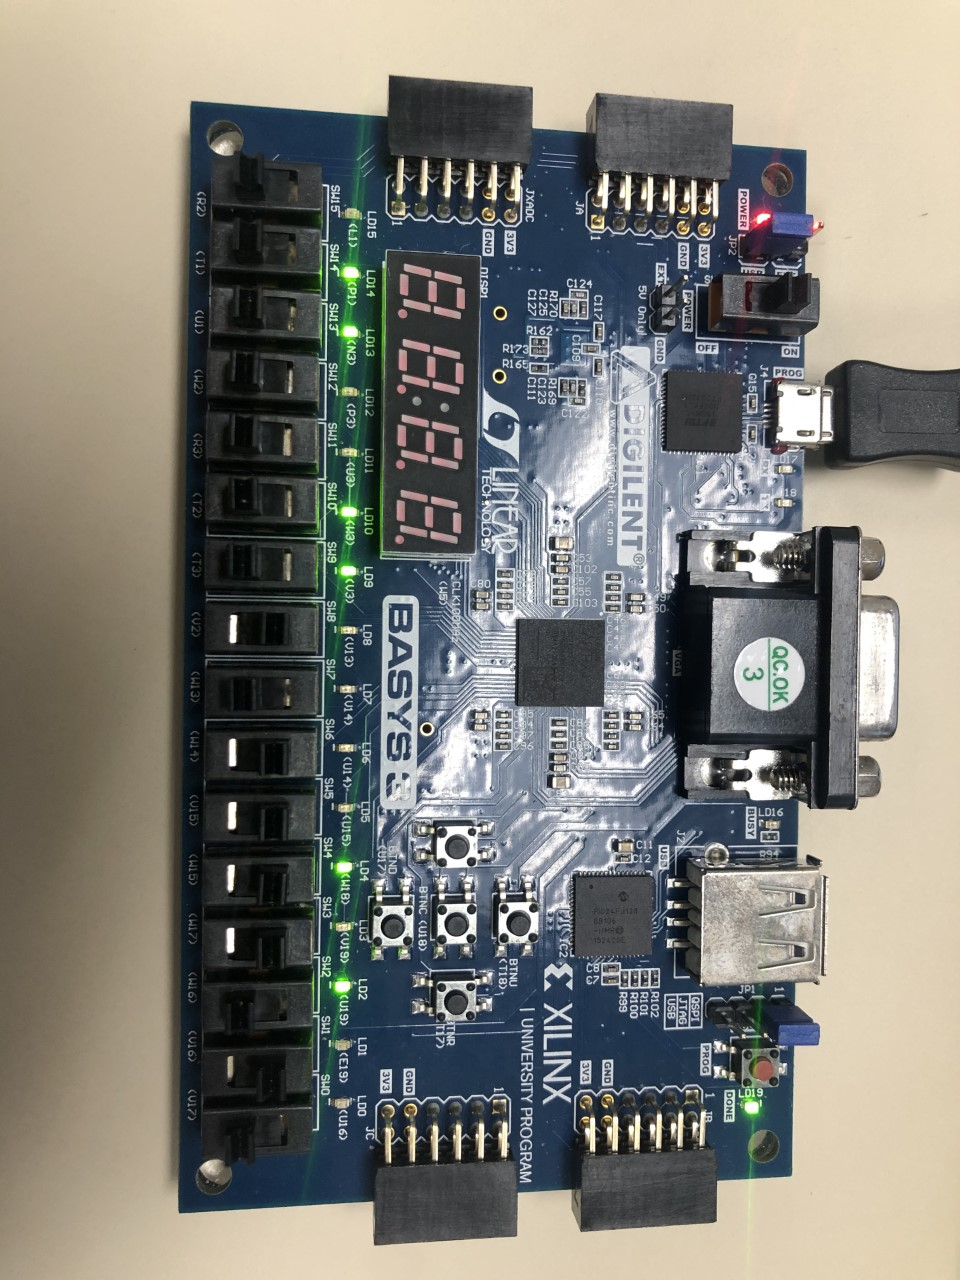
\includegraphics[width= \textwidth ]{bb4.png}
	\caption{register simulation waveform}
	\label{fig: bb4}
\end{figure}

\begin{figure}[ht]\centering
	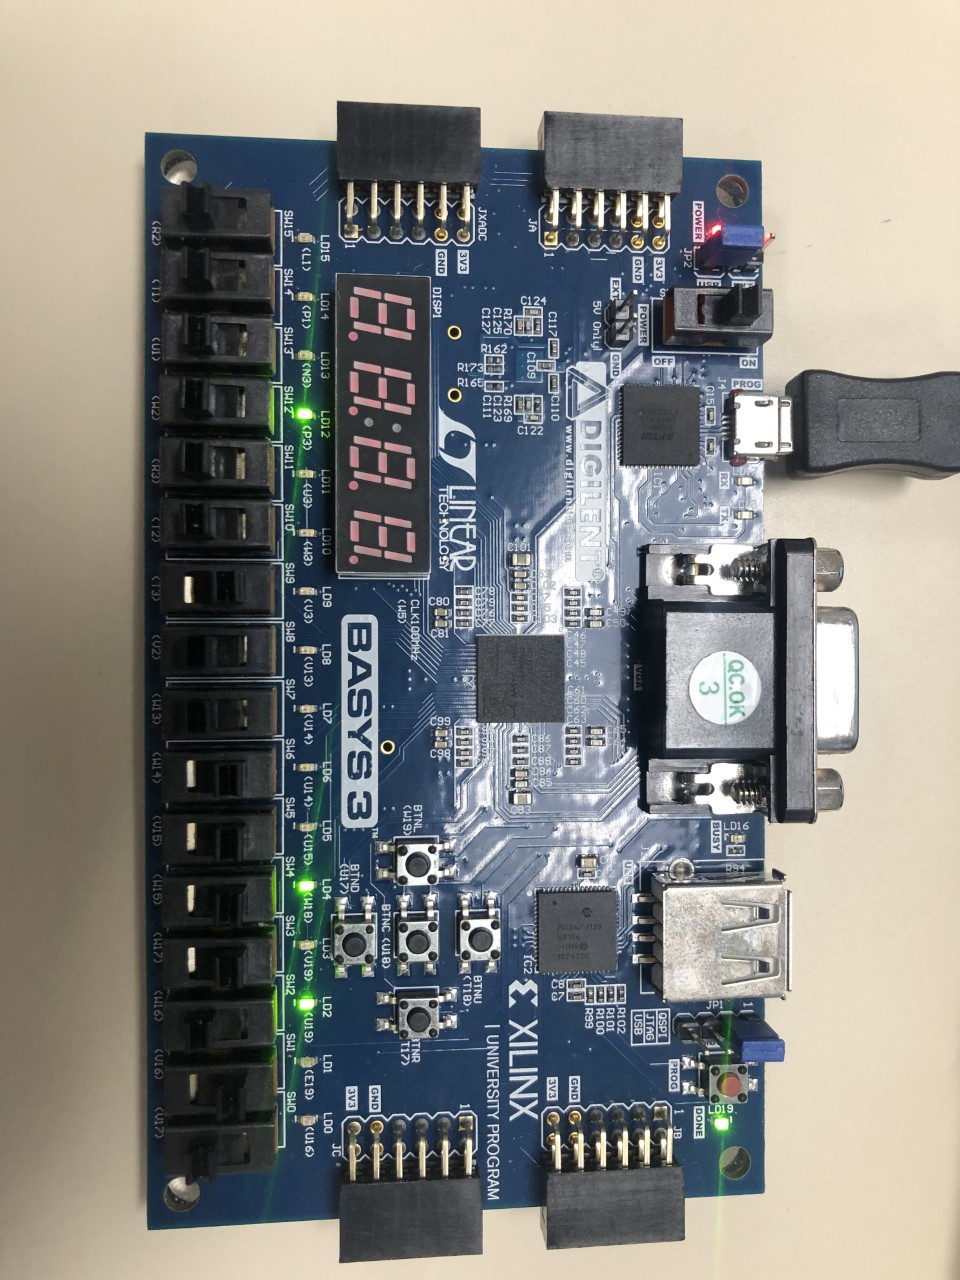
\includegraphics[width= \textwidth ]{bb5.png}
	\caption{register simulation waveform}
	\label{fig: bb5}
\end{figure}
\begin{figure}[ht]\centering
	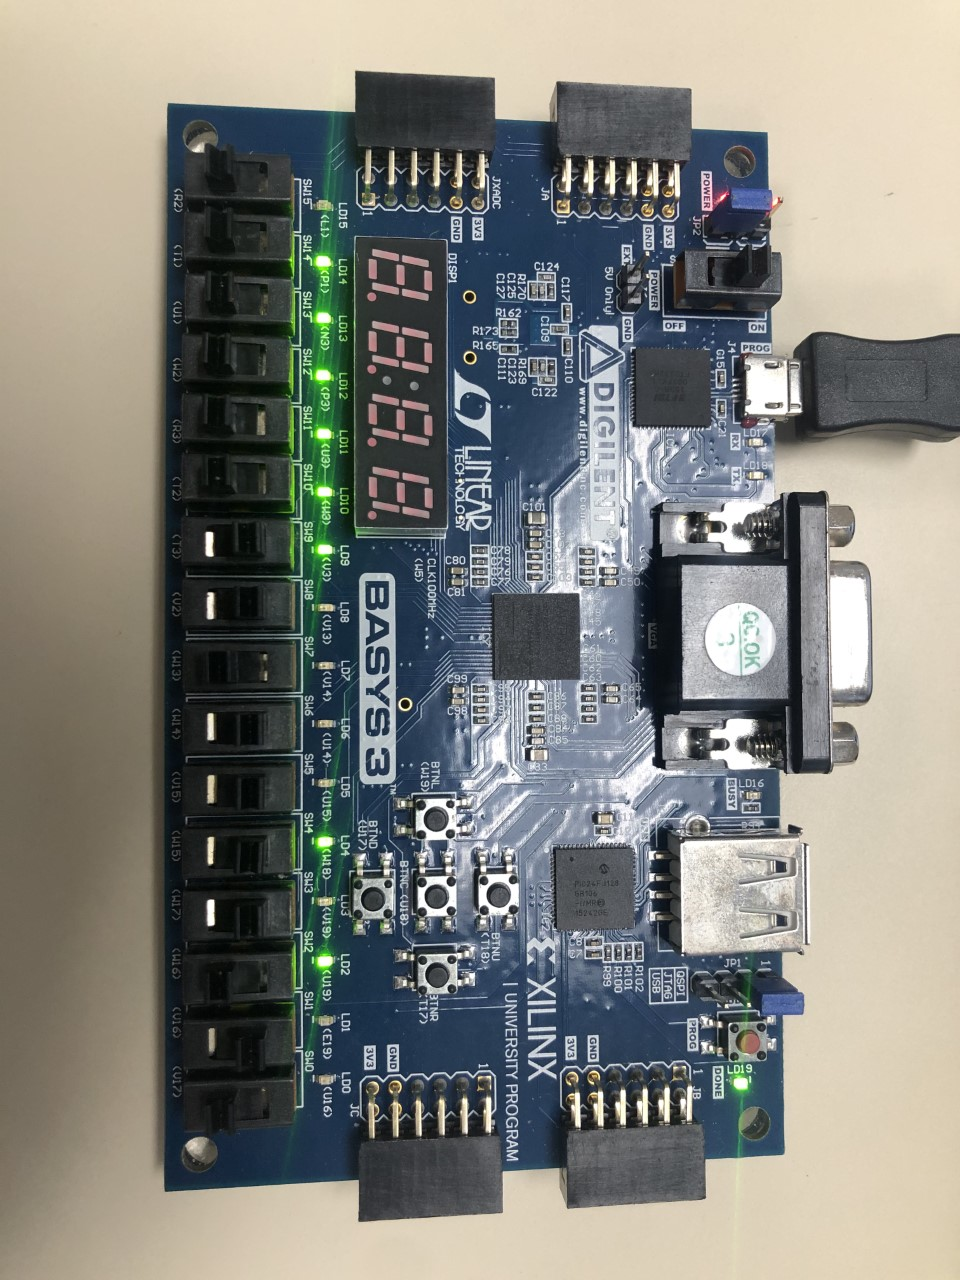
\includegraphics[width= \textwidth ]{bb6.png}
	\caption{register simulation waveform}
	\label{fig: bb6}
\end{figure}
\begin{figure}[ht]\centering
	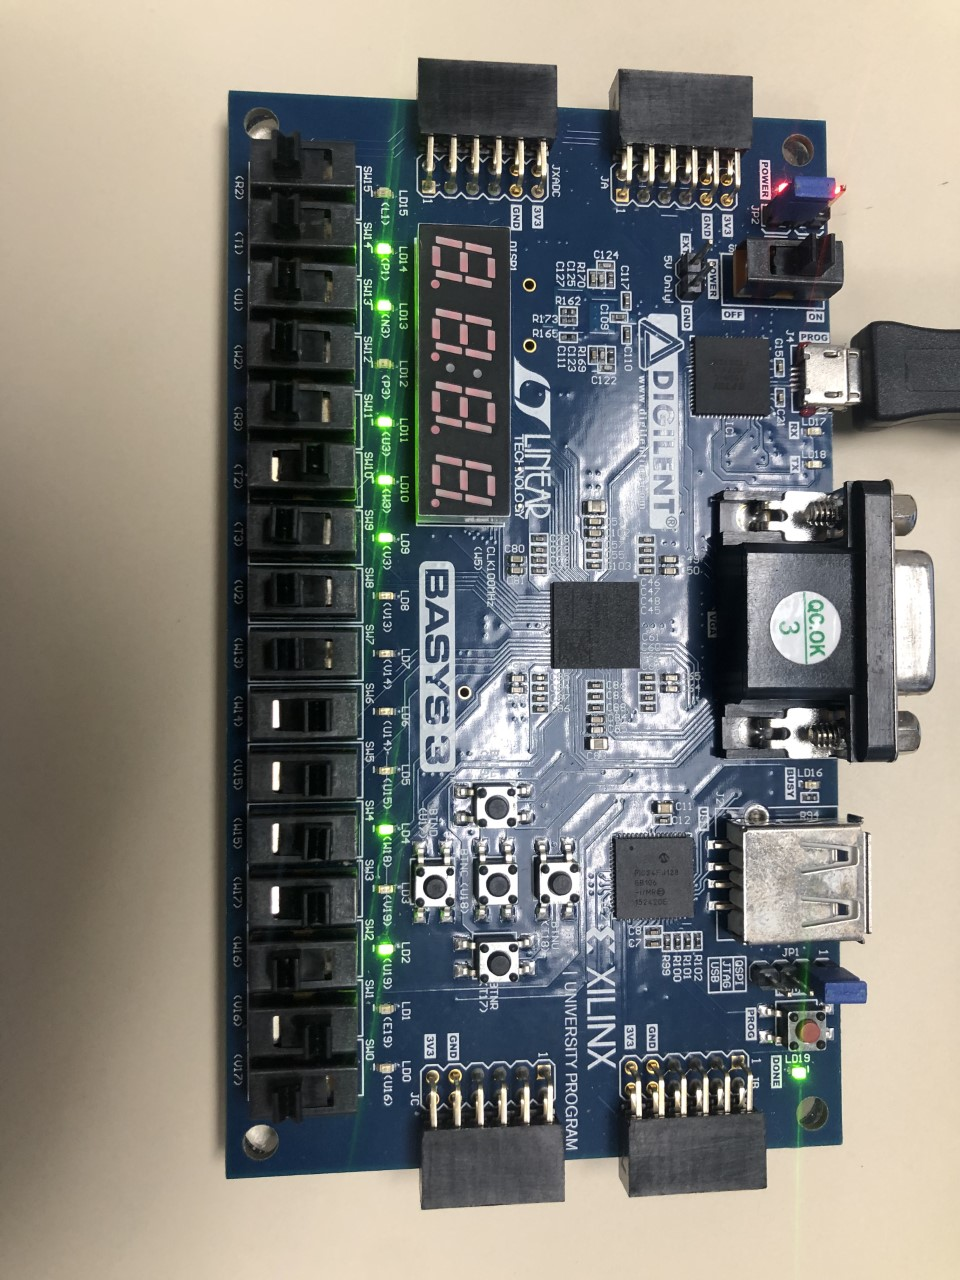
\includegraphics[width= \textwidth ]{bb7.png}
	\caption{register simulation waveform}
	\label{fig: bb7}
\end{figure}
\begin{figure}[ht]\centering
	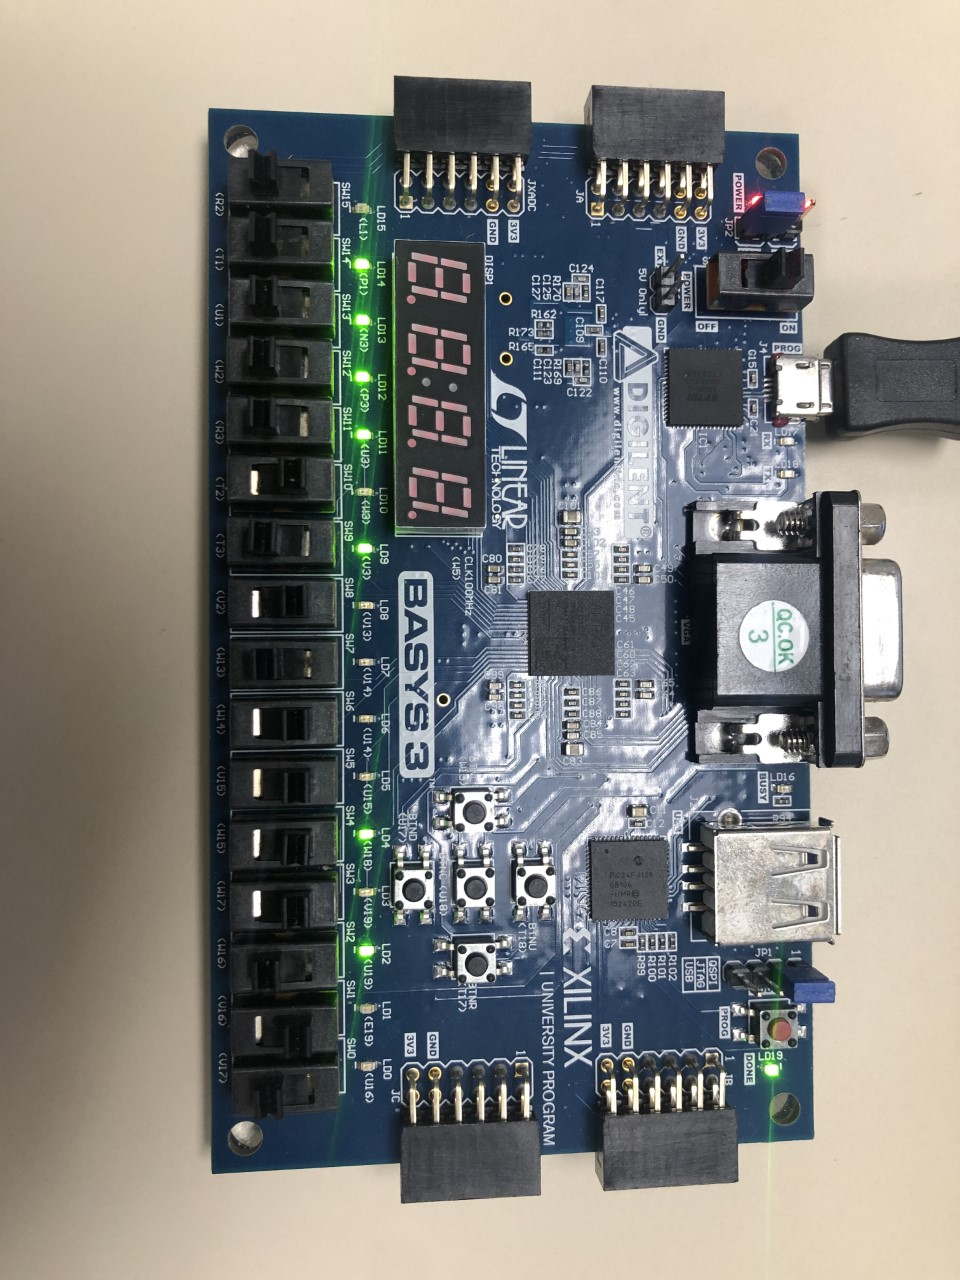
\includegraphics[width= \textwidth ]{bb8.png}
	\caption{register simulation waveform}
	\label{fig: bb8}
\end{figure}
\clearpage
\section*{Expected results tables}

\begin{table*}[ht]\centering
	\caption{\textit{register} expected results table}
	\label{ALU:tbl:register_ERT}\medskip
	\begin{tabular}{l|rrrrrrrrrrr}
		Time (ns): & 0-5 & 5-10 & 10-15 & 15-20 & 20-25 & 25-30 & 30-35 & 35-40 & 40-45 & 45-50 & 50-55 \\
		\midrule
		D (hex) & 0 & 0 	  & A & A & 3 	    & 3 	  & 0 	    & 0 & 0$\to$6 & 6 & 6 \\
		clk     & 0 & 1 	  & 0 & 1 & 0 	    & 1 	  & 0 	    & 1 & 0 	  & 1 & 0 \\
		en  	& 0 & 0 	  & 1 & 1 & 1$\to$0 & 0$\to$1 & 1$\to$0 & 0 & 0$\to$1 & 1 & 1 \\
		rst 	& 0 & 0$\to$1 & 0 & 0 & 0 		& 0 	  & 0		& 0 & 0		  & 0 & 0 \\
		\midrule
		Q (hex) & X & X$\to$0 & A & A & A & A & A & A & 6 & 6 &  6\\
		\bottomrule
	\end{tabular}
\end{table*}

\begin{table*}[ht]\centering
	\caption{\textit{alu} expected results table skeleton}
	\label{ALU:tbl:alu_ERT}\medskip
	\begin{tabular}{l|rrrrrr}
		Time (ns): & 0-10 & 10-20 & 20-30 & 30-40 & 40-50 & 50-60 \\
		\midrule
		in0 0 & 2 & 4 & 8 & 16 & 32 & 34 \\
		in1 0 & 1 & 2 & 3 & 4 & 5 & 6 \\
		op	0 & 1 & 2 & 3 & 4 & 5 & 1 \\
		\midrule
		out 0 & 1 & 0 & 11/b & 12 & 32 & 2e \\
		\bottomrule
	\end{tabular}
\end{table*}



\section*{Code}


\Verilog[caption= register code]{C:/Users/spencer_stinson1/Documents/GitHub/Lab09/Lab_09/Lab_09.srcs/sources_1/new/register.sv}

\Verilog[caption = register testbench code ]{C:/Users/spencer_stinson1/Documents/GitHub/Lab09/Lab_09/Lab_09.srcs/sim_1/new/register_testbench.sv}

\Verilog[caption= alu code]{C:/Users/spencer_stinson1/Documents/GitHub/Lab09/Lab_09/Lab_09.srcs/sources_1/new/alu.sv}

\Verilog[caption = alu testbench code]{C:/Users/spencer_stinson1/Documents/GitHub/Lab09/Lab_09/Lab_09.srcs/sim_2/new/alu_testbench.sv}

\Verilog[caption= top lab9 code]{C:/Users/spencer_stinson1/Documents/GitHub/Lab09/Lab_09/Lab_09.srcs/sources_1/new/top_lab9.sv}

\end{document}
